\chapter{Verwandte Arbeiten}
\label{chap:verwarbeiten}

\section{Unsupervised Image Segmentation by Backpropagation}
\label{sec:kanezaki}
In seinem Paper \cite{kanezaki} stellt Asako Kanezaki einen Ansatz vor, Convolutional Neural Networks zur Bildsegmentierung zu nutzen. Die Besonderheit an diesem Ansatz ist allerdings, dass er nicht wie frühere Versuche CNNs zur Bildsegmentierung zu nutzen auf überwachtem Lernen basiert, sondern unüberwachtes Lernen nutzt.

Dieser Ansatz erstellt eine Mapping-Funktion $c_n=f(x_n)$, die jedem der $N$ $p$-dimensionalen Pixel mit dem Merkmalsvektor $\{x_n\in\mathbb{R}^p\}_{n=1}^N$ eines Eingabebildes ein Clusterlabel $c$ mit $\{c_n\in\mathbb{Z}\}_{n=1}^N$ zuordnet.

Während das Resultat das gleiche wie bei überwachtem Lernen ist, wird hier weder eine Ground Truth, noch ein vorher angelerntes Neuronales Netz benötigt.

Erreicht wird dieses Ziel durch einen iterativen Prozess, in welchem ein anfangs untrainiertes neuronales Netz eine Bildsegmentierung erzeugt, welche anschließend mithilfe einer im Vorhinein erstellten, konstanten Segmentierung optimiert wird. Diese Segmentierung wird in diesem Paper über den SLIC-Algorithmus\cite{slic} erzeugt. Dieser Algorithmus ist in Abbildung~\ref{fig:kanezaki_flowchart} anschaulich dargestellt.

\begin{figure}
	\center{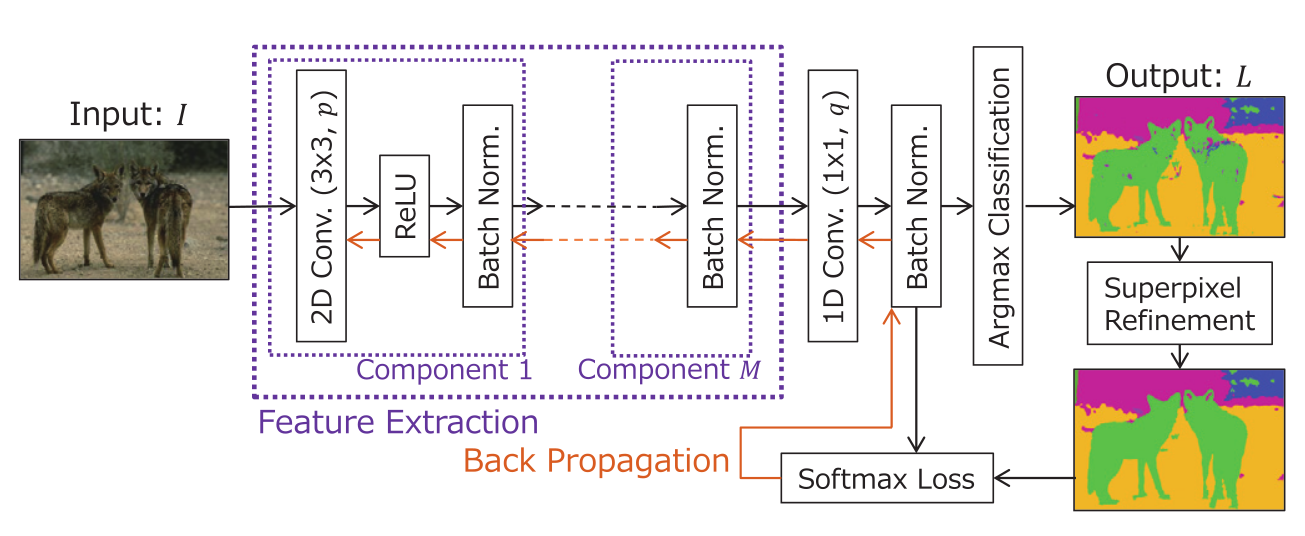
\includegraphics[width=.8\textwidth,keepaspectratio]{images/kanezaki_flowchart.png}}
	\caption{Vorgehensweise nach Kanezaki, aus \cite{kanezaki}}
	\label{fig:kanezaki_flowchart}
\end{figure}

\section{Unsupervised Deep Embedding for Clustering Analysis}
\label{sec:unsupervised_dec}
\cite{unsupervised_dec}

\section{Detection of sub-kilometer craters in high resolution planetary images using shape and texture features}
\label{sec:bandeira}
\cite{bandeira}

\section{Crater Detection via Convolutional Neural Networks}
\label{sec:crater_cnn}
\cite{crater_cnn}